\documentclass{article}
\usepackage{graphicx}
\usepackage{booktabs}
\usepackage[margin=1in]{geometry}
\usepackage{longtable}
\begin{document}

\section*{Results Summary}

\subsection*{Key Input Data and Assumptions}
\begin{table}[ht]
\centering
\begin{tabular}{ll}
\toprule
\textbf{Parameter} & \textbf{Value} \\
\midrule
g0 (m/s²) & 9.81 \\
ISP (Stage 1, Stage 2) & 282, 348 \\
EPSILON (Stage 1, Stage 2) & 0.03, 0.07 \\
Payload Fraction & 0.03 \\
Total ΔV (m/s) & 10500 \\
Gravity Loss (m/s) & 1500 \\
Drag Loss (m/s) & 500 \\
Bounds & [(0.05, 0.85), (0.05, 0.85)] \\
Initial Guess & 0.1, 0.1 \\
\bottomrule
\end{tabular}
\caption{Key Input Parameters}
\end{table}

\subsubsection*{Assumptions}

\begin{enumerate}
    \item The rocket equation is applied in its simplified form.
    \item Structural mass fractions and payload fraction are assumed constant.
    \item The design space is bounded as specified.
    \item The objective function minimizes the squared error between produced and required ΔV.
\end{enumerate}


\subsection*{Solver Performance Summary}
\begin{table}[ht]
\centering
\begin{tabular}{lcccc}
\toprule
\textbf{Solver} & \textbf{Time (s)} & \textbf{Final Error} & \textbf{$\Delta V$ Mismatch (m/s)} & \textbf{Solution Vector} \\
\midrule
SLSQP & 0.0010 & 3.75e+06 & -1935.88 & 0.100, 0.100 \\
Trust-Constr & 0.1947 & 2.21e-08 & 0.00 & 0.053, 0.050 \\
Differential Evolution & 0.3276 & 0.00e+00 & 0.00 & 0.051, 0.052 \\
Genetic Algorithm & 9.1847 & 0.00e+00 & 0.00 & 0.050, 0.054 \\
\bottomrule
\end{tabular}
\caption{Summary of Solver Performance}
\end{table}

\subsection*{Figures}

\begin{figure}[ht]
\centering
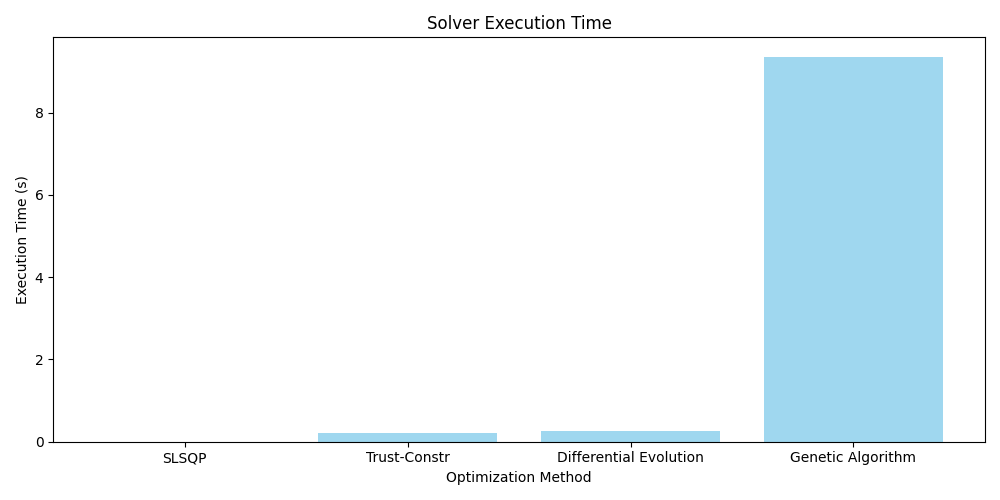
\includegraphics[width=0.8\textwidth]{execution_time.png}
\caption{Execution Time}
\end{figure}

\begin{figure}[ht]
\centering
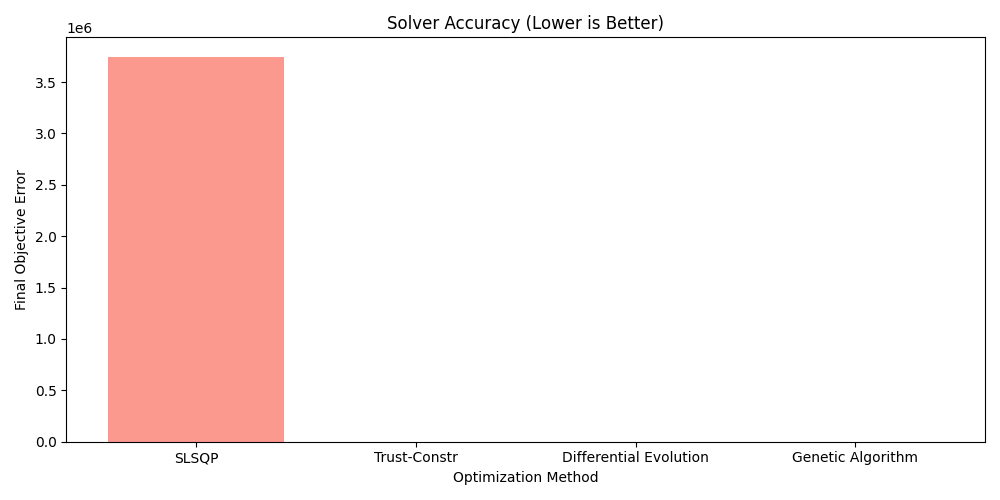
\includegraphics[width=0.8\textwidth]{objective_error.png}
\caption{Final Objective Error}
\end{figure}

\begin{figure}[ht]
\centering
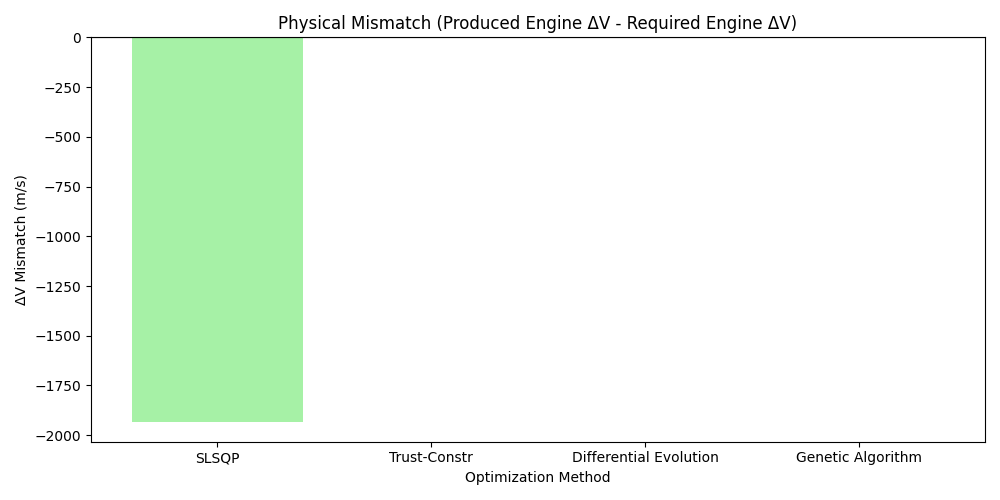
\includegraphics[width=0.8\textwidth]{physical_mismatch.png}
\caption{Physical ΔV Mismatch}
\end{figure}

\begin{figure}[ht]
\centering
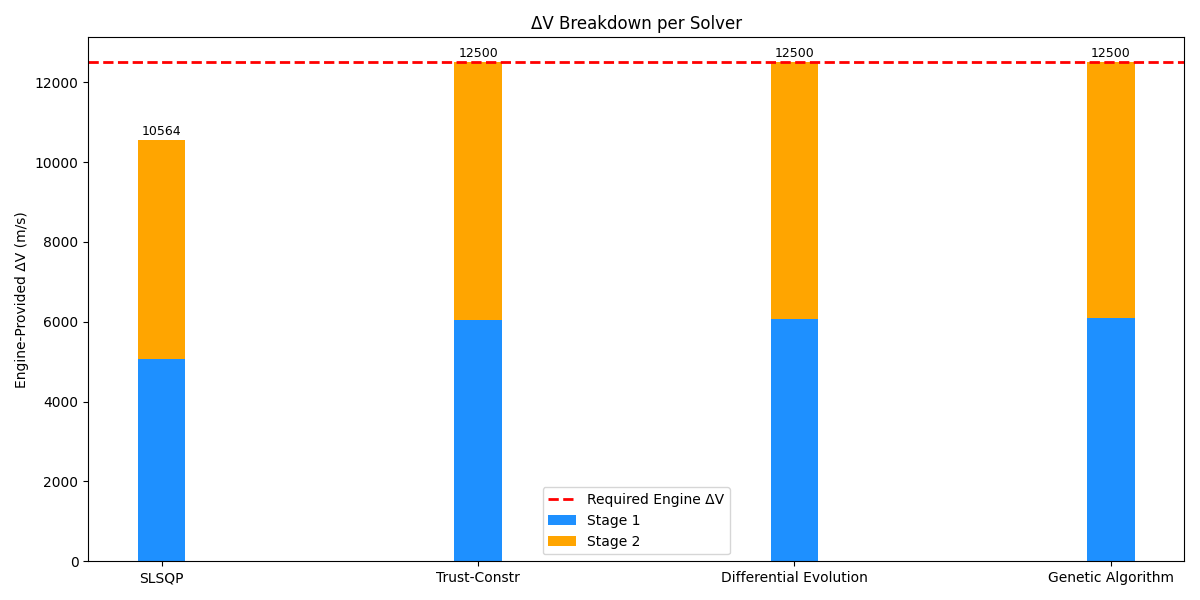
\includegraphics[width=0.8\textwidth]{dv_breakdown.png}
\caption{ΔV Breakdown}
\end{figure}

\begin{figure}[ht]
\centering
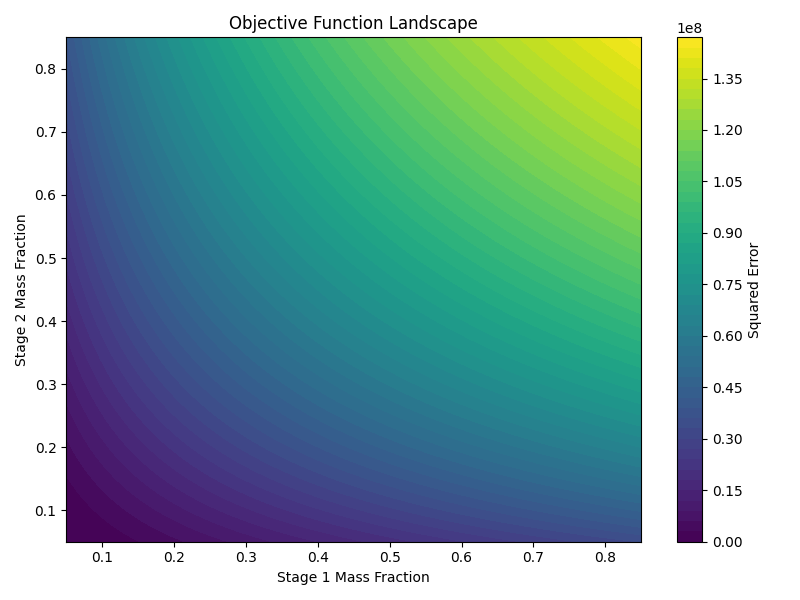
\includegraphics[width=0.8\textwidth]{objective_contour.png}
\caption{Objective Function Contour}
\end{figure}

\begin{figure}[ht]
\centering
\includegraphics[width=0.8\textwidth]{ga_convergence.png}
\caption{GA Convergence Curve}
\end{figure}

\begin{figure}[ht]
\centering
\includegraphics[width=0.8\textwidth]{ga_population_hist.png}
\caption{GA Population Histogram}
\end{figure}
\end{document}